% !TeX root = surgery.tex

\subsection{Manuscripts}
Andrey 
\subsubsection{Features of the manuscript transmission}
Andrey
\subsubsection{Palaeographical features}
\begin{itemize}
    \item śrita for śṛta.
    \item yātri for yātṛ (Su.ka.1.63) % but yātrin is possible
     \item punarṇṇavā  (Su.ka.1.61) % but an old Nepelase ms. of the Brahmayāmala has this spelling.
    \item ś and s in KL 699.
    \item b and v in KL 699 and NAK 5-333.
    \item cha and ccha
    \item line-fillers
    \item \d n for n (punar\d n\d nav\=a)
\end{itemize}

\subsubsection{Chart of characters}

[[[Put a chart from QuickPalaeographer here.]]]

\subsection{The Printed Editions}

The careful survey of printed editions of the \SS\ by Meulenbeld lists no fewer than 
44 entries.\footcite[IIB, 311--314]{meul-hist}  These range from the first edition 
by 
Madhusūdana Gupta (\citeyear{gupt-1835}) to editions in the 1970s. The 
number of 
reprints and editions since that time might almost double that number.  
Translations begin with Hessler's Latin translation in \citeyear{hess-1855} and 
continue up to the present in scores of publications in many 
languages.\footcites[E.g.,][IIB, 314--315]{meul-hist}{zysk-1984}

\subsubsection{The Vulgate}


The great ayurvedic scholar Yādavaśarman Trivikrama Ācārya produced three 
successive editions of the
\SS\ with the commentary of Ḍalhaṇa, in 1915, 1931 and 1938.  These
editions, especially the last, are generally considered the most 
scholarly
and reliable editions of the work, and have been constantly reprinted up
to the present day.\footnote{See also the study of these editions by \textcites[\S 
1.2]{kleb-2021b}[143--144]{wuja-2013}.}  We refer to the last of these editions 
as “the vulgate.”

The 1915 edition was based on three manuscripts.  The 1931 edition used another
seven manuscripts plus two printed editions.  For his final 1938 edition, Ācārya
used a further three manuscripts.\footnote{The following account of the sources is
paraphrased from \citeauthor{vulgate}'s own account of his sources
\citep[22]{vulgate}.}  These sources are described as follow, with an overview in
Table~\ref{tableofeds}.

\subsubsection{The sources of the 1915 edition}

\begin{enumerate}
    \item[1] Calcutta, Royal Asiatic Society.  Covers the \emph{sūtra, nidāna, śārīra 
    and 
        kalpa sthāna}s.  
    
    \item [2] Jaipur, Pandit Gaṅgādharabhaṭṭaśarman, lecturer at the Royal 
    Sanskrit University.  Covers the \emph{cikitsāsthāna} and the 
    \emph{uttaratantra}.
    
    \item [3]  Bundi, my great friend the royal physician Paṃ.\ Śrīprasādaśarman  
    Covers the \emph{uttaratantra}.
\end{enumerate}

\subsubsection{The sources of the 1931 edition}

\begin{enumerate}
    
    \item[1] Vārāṇasī, professor of literature, the great Gaurīnāthapāṭhaka.  With 
    the 
    \emph{Nibandhasaṅgraha}. Covers the \emph{nidānasthāna} and 
    \emph{uttaratantra}.
    
    \item [2]  Ahmedabad.  My friend Sva.\ Vā.\ Vaidya Raṇachoḍalāla 
    Motīlālaśarman.  
    With the \emph{Nibandhasaṅgraha}.  Covers the \emph{śārīrasthāna}.
    
    \item [3] From the personal library of my great friend Sva.\ Vā.\ Vaidya
    Murārajīśarman. Extremely old. No commentary.  Covers the 
    \emph{śārīrasthāna}.
    
    \item [4]  Puṇe, BORI library.  With the \emph{Nibandhasaṅgraha}. Covers the
    \emph{śārīrasthāna}.\footnote{Not one of the three MSS of the
    \emph{śārīrasthāna} described in \cite{shar-vaid}.}
    
    \item [5]  Puṇe, BORI library.  With the \emph{Nibandhasaṅgraha}. Complete.  
    With some damaged folia.
    
    \item [6]  Bombay, Asiatic Society.  Incomplete.\footnote{Possibly 
    \MScite{Mumbai 
    AS B.I.3} or \MScite{Mumbai AS B.D.109} \citep[v.\,1, \# 212 and 
    213]{vela-1930}.  But both these have the \emph{Nibandhasaṅgraha}.  The 
    first 
    covers only the \emph{śārīrasthāna}; the second may be complete, but 
    Velankar calls it 
    only “disorderly.”}
    
    \item [7] Varanasi, the private library of Vaidya Tryambakaśāstrī.  Covers the 
    \emph{cikitsāsthāna}.  The variant readings of this MS were compiled by Prof.\ 
    %    Guruprasādaśāstrī and supplied to Ācārya.
    
    \item [8]  A printed edition together with the commentary 
    \emph{Suśrutasandīpanabhāṣya} by Professor Hārāṇacandra Cakravārtti. 
    Complete work.
    This is the 1910 Calcutta edition numbered “t” by \citet[IB, 
    312]{meul-hist}.\footcite{bhat-1917}
    
    \item [9] A printed edition of the first 43 chapters of the
    \emph{sūtrasthāna}, printed in Bengali script, with the commentaries
    \emph{Bhānumatī}, \emph{Nibandhasaṅgraha}, edited by Vijayaratnasena and
    Niśikāntasena. This is the 1886 Calcutta edition numbered “g” by \citet[IB,
    311]{meul-hist}.\footcite{sena-1886}
    
\end{enumerate}


\subsubsection{The sources of the 1938 edition}
% \coffeestainC{1}{1}{180}{0}{-5 mm}
\begin{enumerate}
    \item [1]  Gwalior, from the library of my great friend Paṃ.\ Rāmeśvaraśāstrin 
    Śukla. 
    Covers the \emph{sūtra, nidāna, śārīra, cikitsā and kalpasthāna}s.
    
   \item[2] Bikaner, from the library of the Royal Palace, supplied by Paṃ.\ 
Candraśekharaśāstrin. Contains the commentary 
\emph{Nyāyacandrikāpañjikāvyākhyā} by Gayadāsa.  Covers the 
\emph{nidānasthāna}.  
%
\begin{table}
   \caption{The sources of Yādavaśarman T. 
    Ācārya's 
    three editions:\\ manuscript coverage (\newmoon) and print coverage
    ($\circ$). \label{tableofeds}}
\vspace{.5\baselineskip}

\begin{tabular}{c|ccc|ccccccccc|ccc}
    \toprule
    %        \multicolumn{16}{c}{\emph{Manuscripts (\newmoon) and print editions 
    %                ($\circ$)}} \\
    \emph{edition}            &\multicolumn{3}{c}{1915}
    &                \multicolumn{9}{c}{1931} 
    &              \multicolumn{3}{c}{1938} \\
    
    \emph{source}         & 1 & 2 & 3 & 1 &2  &3  &4  &5  &6  &7  &8  &9  &1  
    &2 &3 \\
    
    
    \midrule
    
    \emph{sthāna} &&&&&&&&&&&&&&&\\        
    
    \emph{sū}. &  \newmoon&  &  &
    &  &  &  & \newmoon & ? &  & $\circ$ & 
    $\circ$\footnotemark &  
    \newmoon & &\newmoon \\
    
    \emph{ni}. &\newmoon  &  &  &
    \newmoon &  &  &  &  \newmoon&  ?&  & $\circ$ &  &  
    \newmoon&\newmoon & \newmoon\\
    
    \emph{śā}. &  \newmoon&  &  &
    & \newmoon & \newmoon & \newmoon & \newmoon &  ? &  &  
    $\circ$&  &  
    \newmoon& &\newmoon \\
    
    \emph{ci}. &  & \newmoon &  &
    &  &  &  &\newmoon & ? &  \newmoon&$\circ$  &  &
    \newmoon & &\newmoon\footnotemark \\
    
    \emph{ka}.  &\newmoon  &  &  &
    &  &  &  &\newmoon  &  ?&  & $\circ$ &  &  
    \newmoon  & & \\
    
    \emph{utt}.  &  & \newmoon &\newmoon  &
    \newmoon  &  &  &  & \newmoon & ? &  & $\circ$ &  &  
    & & \\
        \bottomrule
\end{tabular}
 \end{table}  
\addtocounter{footnote}{-1}
\footnotetext{Covers chapters 1--43 only.}
\stepcounter{footnote}
\footnotetext{Covers chapters 1--9 only.}
%
This is almost certainly \MScite{Bikaner Anup 
    4390}.\footnote{See Dominik Wujastyk, “MS Bīkāner AnupLib 4390.” 
\emph{Pandit}. 
<\url{http://panditproject.org/entity/108068/manuscript}>.}

\item [3] Kathmandu, located in the private library of the Royal Guru Hemarāja 
Śarman.  An extremely old palm-leaf manuscript. Readings from this MS were 
compiled by Paṃ Nityānandaśarman Jośī and sent to Ācārya. Covers from the 
beginning of the work to the end of the ninth chapter of the 
\emph{cikitsāsthāna}.  The 
siglum for this manuscript in footnotes was \dev{tā} for 
\dev{tālapatrapustake}. 
\end{enumerate}
\subsubsection{Evaluation}

Estimates show that there are approximately 230 extant manuscript
witnesses for the \emph{Suśrutasaṃhitā}.\footnote{This figure is arrived
at by summing the MSS mentioned in \cite{ncc} and in the \cite{ngmcp}. The
real figure could be many scores higher.}  Many of these manuscripts cover only
one or more or its chapters.  Nevertheless, this is an order of magnitude
more evidence than was considered by Ācārya for his vulgate editions.

While the descriptions provided by Ācārya of his source materials seems at first
to be moderately comprehensive, Table~\ref{tableofeds} reveals the underlying
paucity of textual sources for these editions.  At first, it appears that fifteen
manuscripts were consulted.  However, we quickly see that two of the sources 
were
other people's printed editions, and one of those covered less than a quarter of
the work (no.\,9 of 1931).  That reduces the manuscript base to 13 manuscripts.
Ācārya does not appear to have seen two of the manuscripts at all, having been
sent collations prepared for him by others (7 of 1931 and 3 of 1938).  Thus,
Ācārya's final edition was based on the personal consultation of eleven partial
manuscripts.   One of them remains unidentified (6 of 1931). Only a single
manuscript covers the whole of the \emph{Suśrutasaṃhitā}, no.\,5 of the 1931
edition.  Manuscript 1 of 1938 is the next most complete, but it omits the
\emph{uttaratantra}, which comprises a third of the work.  Manuscript 1 of the
1915 edition is third in size, but it still omits both of the longest chapters,
and thus offers less than half the work.  For the rest, the evidence is spotty,
with each part of the work being supported by only between four and eight
manuscripts, excluding the printed editions.

Two sources stand out for their historical importance.  The first is no.\,3 of
1931, which Ācārya calls “extremely old.”  It covered the \emph{śārīrasthāna}
only, and unfortunately we know nothing of the later history of this manuscript.
The second is no.\,3 of 1938, which is one of the important Nepalese manuscripts
being considered in the present project. Ācārya's remarks and references to
Hemarājaśarman's introduction to the \emph{Kāśyapasaṃhitā} allow us
to identify this manuscript as \MScite{Kathmandu NAK 
    5-333}.\footnote{\cites[22]{vulgate}[56--57]{hema-1938}. Discussed by
\citet[\S 1.1, 2.3]{kleb-2021b}.  See also \cites[IIB, 
25--41]{meul-hist}[161--169]{wuja-2003}.} But 
that manuscript covers the whole work, not
just up to the ninth chapter of the \emph{cikitsāsthāna} as
\citeauthor{vulgate} stated.\footcite[22]{vulgate}  Perhaps the editors
only received collations for this portion of the manuscript and did not know that it
was a witness for the whole work.

\subsubsection{The 1939 edition}        

In 1939, Yādavaśarman Trivikrama Ācārya and Nandakiśora Śarman co-edited an
edition of the \emph{sūtrasthāna} of the \emph{Suśrutasaṃhitā} that was 
published
by the Swami Laxmi Ram ayurvedic centre in Jaipur, and printed at the famous
Nirṇayasāgara Press in Mumbai (see 
Fig.\,\ref{bhanumati}).\footnote{\cite{acar-1939}.  The description of 
the sources 
below is based on Yādavaśarman T. Ācārya's  remarks in his introduction 
(pp.\,3--4). See also the remarks on this edition by
\citet[7]{kleb-2021a}.  On the Swami Laxmi Ram
centre, see \cite{hofe-2007}} The text was edited on the basis of the following 
sources.

\begin{figure}[p]
    \centering
    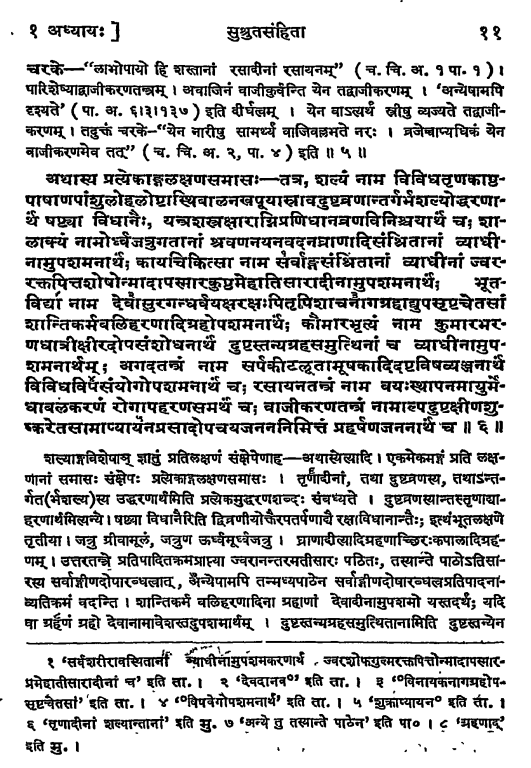
\includegraphics[draft=false,height=.9\textheight]{media/Bhanumati-page-11}
    \caption{A page of the 1939 \emph{Bhānumatī} edition, showing the variant 
        readings in 
        the 
        footnotes.}
    \label{bhanumati}
\end{figure}


\paragraph{For the Bhānumatī}

\begin{enumerate}
    \item A printed edition.  Covered the \emph{Bhānumatī} up to chapter Su.sū.40.
    The siglum was \dev{mu} for \emph{mudrita}.\footnote{\cite{sena-1886}.  
    The
    manuscript on which this edition was based is probably in the library of the
    Calcutta Sanskrit College, and described in \cite[v.\,X.1]{sast-1917}, which
    is not available to me.  See also \cite[IB, 495, n.\,57]{meul-hist} for
    mention of this manuscript.  The reference at \cite[217]{rao-sans} to CSCL
    accession number 97 in Bengali script may be this manuscript.}
    
    \item A manuscript in the India Office Library library provided through the
    Bhandarkar Oriental Research Institute in Pune.\footnote{At this time,
    manuscripts from Britain were routinely lent to scholars in India and vice
    versa.} This manuscript covered the \emph{Bhānumatī} b up to the end of the
    \emph{sūtrasthāna}.  The siglum was \dev{ha} for
    \dev{hastalikhita}.\footnote{\cite{PP109978}\\ 
    \MScite{London BL H. T. Colebrooke 908}
    (\href{panditproject.org/entity/109978/manuscript}{PanditProject \#109978},
    consulted on July 03, 2021).}
\end{enumerate}

\paragraph{For the Suśrutasaṃhitā}

\begin{enumerate}
    \item A palm leaf manuscript from Hemarājaśarman's personal
    library.\footnote{I.e., \MScite{Kathmandu NAK 5-333}.}  The siglum was
    \dev{tā} for \dev{tāḍapatra}.
    
    \item His own published edition. The siglum was \dev{ḍa} for 
    \dev{ḍalhaṇasaṃmataḥ
        pāṭhaḥ}.\footnote{\cite{vulgate}.  It is noteworthy that Ācārya refers to
    his 1938 edition as representing “the Ḍalhaṇa recension.”}
    
    \item Hārāṇacandra Cakravarti's published edition with his own
    commentary.\footcite{bhat-1917} The siglum was \dev{hā}.
\end{enumerate}
%
\subsubsection{Evaluation}

The main innovation of this publication was to present the only surviving part of
the commentary on the \SS\ by the great eleventh-century medical scholar
Cakrapāṇidatta, namely the \emph{Bhānumatī}.\footcite[IA, 374--375 and IB,
495--496]{meul-hist} A secondary purpose was to present the text of the
\emph{sūtrasthāna} as read in \MScite{Kathmandu NAK 5-333}, that had recently 
been
brought to the editors' attention. In their judgement, the Kathmandu manuscript
presented a text that was closer to what Cakrapāṇidatta had before him than the
text according to Ḍalhaṇa.   This was the first \SS\ edition in which Ācārya used
sigla to identify the sources from which variant readings were reported, so while
it has limitations, it for the first time enables us to get some idea of origins
of the text (see Figure~\ref{bhanumati}).

Ācārya noted in his introduction that the manuscripts containing the Ḍalhaṇa's
commentary all came together with the root-text of the \SS, and thus the main \SS\
text reflected the readings chosen by Ḍalhaṇa.  But the manuscripts of the
\emph{Bhānumatī} contained the commentary alone, without the root-text, and 
had
many explanations based on different readings of the root-text than those of
Ḍalhaṇa.  In many of these cases it was hard to know what the text that
Cakrapāṇidatta had before him. But Ācārya noted that Cakrapāṇidatta had a text
before him that had much in common with the text of the Nepalese
manuscript.\footnote{\cite[3--4]{acar-1939}.  See discussion by
\citet[7]{kleb-2021a}.}  

There is compelling evidence that Cakrapāṇidattas's \emph{Bhānumatī} 
commentary
once covered the whole text of the \SS.\footcite[IA, 375]{meul-hist}  The loss of
the rest of the work ranks amongst the greatest disasters in Āyurvedic
literature.  Remarkably, the whole \emph{Bhānumatī} may still have existed in the
early twentieth century. In 1903, Palmyr Cordier reported being privately informed
of a complete copy of the work in a personal manuscript collection in
Benares.\footcite[332]{cord-1903}
   
\subsection{Editorial Principles}
\subsubsection{Method}
The data for the critical edition comes from the witnesses of the Nepalese version, which are primarily the manuscripts that have been described above. Diplomatic transcriptions of SS.1.16 of these manuscripts have been created by researchers of the Suśruta Project\footnote{https://sushrutaproject.org, accessed 20/8/2021.} according to a subset of TEI Guidelines that has been formulated by Charles Li.\footnote{These guidelines are at https://saktumiva.org/wiki/tei, accessed 20/10/2021.} MS NAK 5-333 is usually transcribed first because the script is easy to read, the scans are clear, and it is the most complete of the manuscript witnesses. Then, MS KL 699 and MS NAK 1-1079 are transcribed. 

The diplomatic transcripts are uploaded to Charles Li's platform Saktumiva.org, where they are automatically collated. An electronic text of the vulgate of the \SS\ without the commentaries, which was transcribed by Tsutomu Yamashita and Yasutaka Muroya on the basis of Ācārya's 1931 and 1938 Bombay editions,\footnote{This e-text is available on the SARIT website; https://sarit.indology.info/susrutasamhita.xml?view=div, accessed 20/8/2021.} was also collated. This enables Project researchers to compare the Nepalese version with the vulgate, the variant readings and additional text of which appears in the critical apparatus.

Saktumiva's automatic collation function standardises punctuation and orthographic variants according to filters which can be turned off or on. These filters enable the editors to ignore \emph{daṇḍa}s, numbers and \emph{puṣpikā}s in the transcripts, as well as orthographic variants, such as \emph{ba} and \emph{va}, certain germinated consonants, and \emph{visarga} variants. A provisional edition of SS.1.16 was created by Jason Birch from the automatic collation, which the project's researchers read together at weekly seminars. Manuscript images were routinely checked to verify the transcripts, particularly when a reading was uncertain; the commentaries of Cakrapāṇidatta and Ḍalhaṇa were read, and variant readings reported by these commentators were included in notes to the edition; and various reference books were consulted, such as the  \citet{josi-maha,nadk-1954} and \citet{meul-hist}, to elucidate the meaning of technical terms, identify relevant information in other medical works and the like. 

An initial draft of the translation and many of the annotations were created from the researchers' discussions of the text's meaning during the seminars, and were recorded by Dominic Wujastyk. The transcripts, provisional edition and translation were uploaded to the project's repository at Github on a weekly basis. Therefore, the project's work is publicly available as it evolves. The following software tools have been selected by Wujastyk for the procedures described above: 

\begin{enumerate}
    \item
    oXygen XML editor (which has plugins for Github and TEI, and can validate the code).\footnote{https://www.oxygenxml.com.}
    
       \item
        Saktumiva (a platform for producing and publishing critical editions of Sanskrit texts).\footnote{http://saktumiva.org.}
        \item
        Quick Palaeographer (a browser-based tool for reading MS images and developing a catalogue of character shapes).\footnote{https://tst.hypotheses.org/1738.}

        \item
        Filezilla (document transfer to Saktumiva).\footnote{https://filezilla-project.org.}       
        \item
        Github (document sharing, security and versioning).\footnote{https://github.com.}   
        \item
         LaTeX (document preparation).\footnote{https://www.latex-project.org.}  
         \item
          qdpm (project management).\footnote{https://qdpm.net.}  
          
\end{enumerate}

\subsubsection{Stemma}
The data from transcripts collated by Saktumiva can be exported as a FASTA file and aligned according to characters, syllables or words by a program called Helayo. The resulting NEXUS file can be read by phylogenetics software to build a stemmatic tree.\footnote{This process is discussed in greater detail by Charles Li at https://chchch.github.io/sanskrit-alignment/docs/index.html#tree, accessed 21/8/2021.} This procedure was done with transcripts of several chapters of the Nepalese witnesses, and the results confirmed our suspicions that K and H are more closely related to one another than K and N. Given the early date of K and the small number of surviving witnesses, the relationship between the manuscripts is reasonably clear and, in the case of SS.1.16, the data was confined to N and H owing to a missing folio of K. The challenge of editing has been to repair the text where it has become corrupt in the few available witnesses. 

\subsubsection{Editing}

\subsubsection{Printed and Digital Outputs}



